\documentclass[a4paper, 11pt]{article}

\usepackage{amsmath}
\usepackage{amssymb}
\usepackage{geometry}
\usepackage{natbib}
\usepackage{graphicx}
\usepackage[utf8]{inputenc}
\usepackage{tikz}
\usepackage[most]{tcolorbox}
\usepackage[backref=page]{hyperref}


\definecolor{antiquewhite}{rgb}{0.98, 0.92, 0.84}

\newtcbtheorem{Takeaway}{\bfseries Takeaway}{enhanced,
  coltitle=black,
  top=0.3in,
  colback=antiquewhite,
  attach boxed title to top left=
  {xshift=1.5em,yshift=-\tcboxedtitleheight/2},
  boxed title style={size=small,colback=pink}
}{Takeaway}

\geometry{left=1.5cm, top=1.5cm, right=1.5cm, bottom=2cm, footskip=.5cm} 
%dvips -Ppdf -tletter -G0 -o paper.ps paper.dvi


\newcommand{\A}{\mathbb{A}}
\newcommand{\B}{\mathbb{B}}
\newcommand{\C}{\mathbb{C}}
\newcommand{\D}{\mathbb{D}}
\newcommand{\E}{\mathbb{E}}
\newcommand{\F}{\mathbb{F}}
\newcommand{\G}{\mathbb{G}}
\newcommand{\Hh}{\mathbb{H}} 
\newcommand{\I}{\mathbb{I}}
\newcommand{\J}{\mathbb{J}}
\newcommand{\K}{\mathbb{K}}
\newcommand{\M}{\mathbb{M}}
\newcommand{\N}{\mathbb{N}}
% \newcommand{\P}{\mathbb{P}}
\newcommand{\Q}{\mathbb{Q}}
\newcommand{\R}{\mathbb{R}}
% \newcommand{\S}{\mathbb{S}}
\newcommand{\T}{\mathbb{T}}
\newcommand{\U}{\mathbb{U}}
\newcommand{\V}{\mathbb{V}}
\newcommand{\W}{\mathbb{W}}
\newcommand{\X}{\mathbb{X}}
\newcommand{\Y}{\mathbb{Y}}
\newcommand{\Z}{\mathbb{Z}}


\newcommand{\x}{\times}



%*********For chapter on binary and categorical data***********
\newcommand{\tvx}{\widetilde{\vx}}
\newcommand{\tvX}{\widetilde{\vX}}
\newcommand{\deriv}[2]{\frac{\partial{#1}}{\partial{#2}}}
\newcommand{\secondderiv}[2]{\frac{\partial^2{#1}}{\partial{#2}^2}}
\newcommand{\neglvb}{\overline{f}}
\newcommand{\bv}{\overline{v}}
\newcommand{\bvm}{\overline{\vm}}
\newcommand{\bvv}{\overline{\vv}}
\newcommand{\bvV}{\overline{\vV}}
\newcommand{\tmu}{\widetilde{\vmu}}
\newcommand{\tSigma}{\widetilde{\vSigma}}
\newcommand{\tm}{\widetilde{m}}
\newcommand{\tv}{\widetilde{v}}
\newcommand{\tsigma}{\widetilde{\sigma}}
\newcommand{\tV}{\widetilde{V}}
\newcommand{\tvSigma}{\widetilde{\vSigma}}
\newcommand{\tg}{\widetilde{\gamma}}
\newcommand{\tvm}{\widetilde{\vm}}
\newcommand{\tvv}{\widetilde{\vv}}
\newcommand{\tvV}{\widetilde{\vV}}
\newcommand{\tvLambda}{\widetilde{\vLambda}}
\newcommand{\tvlambda}{\widetilde{\vlambda}}
\newcommand{\tlambda}{\widetilde{\lambda}}
\newcommand{\tvgamma}{\widetilde{\vgamma}}
\newcommand{\tgamma}{\widetilde{\gamma}}
\newcommand{\teta}{\widetilde{\eta}}
\newcommand{\tphi}{\widetilde{\phi}}

\newcommand{\talpha}{\widetilde{\alpha}}
\newcommand{\tvg}{\widetilde{\vg}}
\newcommand{\tvh}{\widetilde{\vh}}
\newcommand{\tvH}{\widetilde{\vH}}
\newcommand{\tvP}{\widetilde{\vP}}
\newcommand{\tvG}{\widetilde{\vG}}
\newcommand{\tvA}{\widetilde{\vA}}
\newcommand{\tp}{\tilde{p}}
%\newcommand{\lse}{\mbox{llp}}
%\usepackage{algorithm}

% numbers a line in align* block
\newcommand\numberthis{\addtocounter{equation}{1}\tag{\theequation}}


%% densify spacing in bibliographies
\newcommand{\bibfix}{%    PUT \bibfix in file.bbl after first line
    \setlength{\parsep}{\parskip}%
    \setlength{\itemsep}{0cm}%
    \setlength{\topsep}{\parskip}%
    \setlength{\parskip}{0cm}%
    \setlength{\partopsep}{0cm}%
    \setlength{\listparindent}{\parindent}%
    \setlength{\labelwidth}{10pt}%
    \setlength{\labelsep}{0pt}%
    \setlength{\leftskip}{0pt}%
    \setlength{\leftmargin}{0pt}%
}


\newtheorem{claim}{Claim}{}
\newtheorem{thm}{Theorem}{}
\newtheorem{prop}{Proposition}{}
\newtheorem{corr}{Corollary}{}
%\newtheorem{lemma}{Lemma}{}
\newtheorem{defn}{Definition}{}
\newenvironment{mythm}{{\bf Theorem}}{}
\newenvironment{myproof}{{\bf Proof}}{}


\newcommand{\choice}[2]{\left(\!\!\! \begin{array}{c} #1 \\ #2\end{array} \!\!\!\right)}
\newcommand{\half}{\mbox{$\frac{1}{2}$}}
\newcommand{\defeq}{\stackrel{\rm def}{=}}
%\newcommand{\defeq}{\mbox{$\stackrel{\rm def}{=}}$}
%\newcommand{\real}{{\rm I\hspace{-0.2em}R}}
\newcommand{\lra}{\mbox{$\leftrightarrow$}}
\newcommand{\Ra}{\mbox{$\Rightarrow$}}
\newcommand{\la}{\mbox{$\leftarrow$}}
\newcommand{\tr}{\mbox{$\mbox{tr}$}}
%\newcommand{\det}{\mbox{$\mbox{det}$}}

\newcommand{\rnd}[1]{\left(#1\right)}
\newcommand{\sqr}[1]{\left[#1\right]}
\newcommand{\crl}[1]{\left\{#1\right\}}
\newcommand{\myang}[1]{\langle#1\rangle}


\newcommand{\range}{\mbox{$\mbox{range}$}}
\newcommand{\myspan}{\mbox{$\mbox{span}$}}
\newcommand{\nullspace}{\mbox{$\mbox{nullspace}$}}
\newcommand{\adj}{\mbox{$\mbox{adj}$}}
\newcommand{\nbd}{\mbox{$\mbox{nbd}$}}



\newcommand{\define}[1]{{\bf #1}}


%\newcommand{\keyword}[1]{{\bf #1}}
\newcommand{\keyword}[1]{{\bf #1}\index{keywords}{#1}}
\newcommand{\addtoindex}[1]{#1 \index{keywords}{#1}}
\newcommand{\keywordSpecial}[2]{{\bf #1}\index{keywords}{#2@#1}}
\newcommand{\bfidx}[1]{{\bf #1}}
\newcommand{\keywordDef}[1]{{\bf #1}\index{keywords}{#1|bfidx}}
%\newcommand{\keyworddef}[1]{{\bf #1}\index{keywords}{#1@{\bf #1}}}
\newcommand{\codename}[1]{{\tt #1}\index{code}{#1}}
\newcommand{\netlabname}[1]{{\tt #1}}
\newcommand{\Rcmd}[1]{{\tt #1}}
\newcommand{\matlabcmd}[1]{{\tt #1}}
\newcommand{\matlabscript}[1]{{\tt #1}}
\newcommand{\dataname}[1]{{\tt #1}}

%\newcommand{\dim}{\mbox{dim}}
\newcommand{\softmax}{\calS}
%\newcommand{\softmax}{\mbox{softmax}}
\newcommand{\sign}{\mbox{sign}}
\newcommand{\iid}{\mbox{iid}}
\newcommand{\mle}{\mbox{mle}}
\newcommand{\myiff}{\mbox{iff}}
\newcommand{\pd}{\mbox{pd}}
\newcommand{\pdf}{\mbox{pdf }}
\newcommand{\cdf}{\mbox{cdf}}
\newcommand{\pmf}{\mbox{pmf}}
\newcommand{\wrt}{\mbox{wrt}}
\newcommand{\MLABA}{\mbox{FML}}
\newcommand{\mywp}{\mbox{wp}}

\newcommand{\myvec}[1]{\mbox{$\mathbf{#1}$}}
\newcommand{\myvecsym}[1]{\mbox{$\boldsymbol{#1}$}}

\newcommand{\vzero}{\mbox{$\myvecsym{0}$}}
\newcommand{\vone}{\mbox{$\myvecsym{1}$}}

\newcommand{\valpha}{\mbox{$\myvecsym{\alpha}$}}
\newcommand{\vbeta}{\mbox{$\myvecsym{\beta}$}}
\newcommand{\vchi}{\mbox{$\myvecsym{\chi}$}}
\newcommand{\vdelta}{\mbox{$\myvecsym{\delta}$}}
\newcommand{\vDelta}{\mbox{$\myvecsym{\Delta}$}}
\newcommand{\vepsilon}{\mbox{$\myvecsym{\epsilon}$}}
\newcommand{\veta}{\mbox{$\myvecsym{\eta}$}}
\newcommand{\vgamma}{\mbox{$\myvecsym{\gamma}$}}
\newcommand{\vmu}{\mbox{$\myvecsym{\mu}$}}
\newcommand{\vlambda}{\mbox{$\myvecsym{\lambda}$}}
\newcommand{\vLambda}{\mbox{$\myvecsym{\Lambda}$}}
\newcommand{\vLambdaBar}{\mbox{$\overline{\vLambda}$}}
\newcommand{\vrho}{\mbox{$\myvecsym{\rho}$}}
\newcommand{\vphi}{\mbox{$\myvecsym{\phi}$}}
\newcommand{\vPhi}{\mbox{$\myvecsym{\Phi}$}}
\newcommand{\vpi}{\mbox{$\myvecsym{\pi}$}}
\newcommand{\vpsi}{\myvecsym{\psi}}
\newcommand{\vPsi}{\mbox{$\myvecsym{\Psi}$}}
\newcommand{\vtheta}{\mbox{$\myvecsym{\theta}$}}
\newcommand{\vTheta}{\mbox{$\myvecsym{\Theta}$}}
\newcommand{\vsigma}{\mbox{$\myvecsym{\sigma}$}}
\newcommand{\vSigma}{\mbox{$\myvecsym{\Sigma}$}}
\newcommand{\vOmega}{\mbox{$\myvecsym{\Omega}$}}
\newcommand{\vtau}{\mbox{$\myvecsym{\tau}$}}
\newcommand{\vxi}{\mbox{$\myvecsym{\xi}$}}

\newcommand{\va}{\mbox{$\myvec{a}$}}
\newcommand{\vb}{\mbox{$\myvec{b}$}}
\newcommand{\vc}{\mbox{$\myvec{c}$}}
\newcommand{\vd}{\mbox{$\myvec{d}$}}
\newcommand{\ve}{\mbox{$\myvec{e}$}}
\newcommand{\vo}{\mbox{$\myvec{o}$}}
\newcommand{\vi}{\mbox{$\myvec{i}$}}
\newcommand{\vf}{\mbox{$\myvec{f}$}}
\newcommand{\vg}{\mbox{$\myvec{g}$}}
\newcommand{\vh}{\mbox{$\myvec{h}$}}
\newcommand{\vj}{\mbox{$\myvec{j}$}}
\newcommand{\vk}{\mbox{$\myvec{k}$}}
\newcommand{\vm}{\mbox{$\myvec{m}$}}
\newcommand{\vn}{\mbox{$\myvec{n}$}}
\newcommand{\vp}{\mbox{$\myvec{p}$}}
\newcommand{\vq}{\mbox{$\myvec{q}$}}
\newcommand{\vr}{\mbox{$\myvec{r}$}}
\newcommand{\vs}{\mbox{$\myvec{s}$}}
\newcommand{\vt}{\mbox{$\myvec{t}$}}
\newcommand{\vu}{\mbox{$\myvec{u}$}}
\newcommand{\vv}{\mbox{$\myvec{v}$}}
\newcommand{\vw}{\mbox{$\myvec{w}$}}
\newcommand{\vws}{\mbox{$\vw_s$}}
\newcommand{\vwh}{\mbox{$\hat{\vw}$}}
\newcommand{\vx}{\mbox{$\myvec{x}$}}
\newcommand{\vxt}{\mbox{$\myvec{\tilde{x}}$}}
\newcommand{\vy}{\mbox{$\myvec{y}$}}
\newcommand{\vyt}{\mbox{$\myvec{\tilde{y}}$}}
\newcommand{\vz}{\mbox{$\myvec{z}$}}
\newcommand{\vA}{\mbox{$\myvec{A}$}}
\newcommand{\vB}{\mbox{$\myvec{B}$}}
\newcommand{\vC}{\mbox{$\myvec{C}$}}
\newcommand{\vD}{\mbox{$\myvec{D}$}}
\newcommand{\vE}{\mbox{$\myvec{E}$}}
\newcommand{\vF}{\mbox{$\myvec{F}$}}
\newcommand{\vG}{\mbox{$\myvec{G}$}}
\newcommand{\vH}{\mbox{$\myvec{H}$}}
\newcommand{\vI}{\mbox{$\myvec{I}$}}
\newcommand{\vJ}{\mbox{$\myvec{J}$}}
\newcommand{\vK}{\mbox{$\myvec{K}$}}
\newcommand{\vL}{\mbox{$\myvec{L}$}}
\newcommand{\vM}{\mbox{$\myvec{M}$}}
\newcommand{\vN}{\mbox{$\myvec{N}$}}
\newcommand{\vO}{\mbox{$\myvec{O}$}}
\newcommand{\vP}{\mbox{$\myvec{P}$}}
\newcommand{\vQ}{\mbox{$\myvec{Q}$}}
\newcommand{\vR}{\mbox{$\myvec{R}$}}
\newcommand{\vS}{\mbox{$\myvec{S}$}}
\newcommand{\vT}{\mbox{$\myvec{T}$}}
\newcommand{\vU}{\mbox{$\myvec{U}$}}
\newcommand{\vV}{\mbox{$\myvec{V}$}}
\newcommand{\vW}{\mbox{$\myvec{W}$}}
\newcommand{\vX}{\mbox{$\myvec{X}$}}
%\newcommand{\vXs}{\mbox{$\vX_{\vs}$}}
\newcommand{\vXs}{\mbox{$\vX_{s}$}}
\newcommand{\vXt}{\mbox{$\myvec{\tilde{X}}$}}
\newcommand{\vY}{\mbox{$\myvec{Y}$}}
\newcommand{\vZ}{\mbox{$\myvec{Z}$}}



\newcommand{\precw}{\mbox{$\lambda_{w}$}} % precision of weights (alpha)
\newcommand{\precy}{\mbox{$\lambda_{y}$}} % precision of y (beta)
\newcommand{\fbar}{\mbox{$\overline{f}$}}
\newcommand{\xbar}{\mbox{$\overline{x}$}}
\newcommand{\ybar}{\mbox{$\overline{y}$}}
\newcommand{\vxbar}{\mbox{$\overline{\vx}$}}
\newcommand{\vybar}{\mbox{$\overline{\vy}$}}
\newcommand{\Xbar}{\mbox{$\overline{X}$}}
\newcommand{\Ybar}{\mbox{$\overline{Y}$}}
\newcommand{\Jbar}{\mbox{$\overline{J}$}}
\newcommand{\Lbar}{\mbox{$\overline{L}$}}
\newcommand{\Tbar}{\mbox{$\overline{T}$}}

\newcommand{\htilde}{\mbox{$\tilde{h}$}}
\newcommand{\vhtilde}{\mbox{$\tilde{\vh}$}}
\newcommand{\Dtilde}{\mbox{$\tilde{D}$}}
\newcommand{\wtilde}{\mbox{$\tilde{w}$}}
\newcommand{\xtilde}{\mbox{$\tilde{x}$}}
\newcommand{\Xtilde}{\mbox{$\tilde{X}$}}
\newcommand{\ytilde}{\mbox{$\tilde{y}$}}
\newcommand{\Ytilde}{\mbox{$\tilde{Y}$}}
\newcommand{\vxtilde}{\mbox{$\tilde{\vx}$}}
\newcommand{\vytilde}{\mbox{$\tilde{\vy}$}}
\newcommand{\ztilde}{\mbox{$\tilde{\z}$}}
\newcommand{\vztilde}{\mbox{$\tilde{\vz}$}}
\newcommand{\vthetaMAP}{\mbox{$\hat{\vtheta}_{MAP}$}}
\newcommand{\vthetahat}{\mbox{$\hat{\vtheta}$}}
\newcommand{\thetahat}{\mbox{$\hat{\theta}$}}
\newcommand{\thetabar}{\mbox{$\overline{\theta}$}}
\newcommand{\vthetabar}{\mbox{$\overline{\vtheta}$}}
\newcommand{\pibar}{\mbox{$\overline{\pi}$}}
\newcommand{\vpibar}{\mbox{$\overline{\vpi}$}}


\newcommand{\sss}{\mbox{$s^2$}}
\newcommand{\vvv}{\mbox{$v$}}
\newcommand{\RSS}{\mbox{RSS}}

%\newcommand{\do}{\mbox{$\mbox{do}$}}

%\newcommand{\xdi}{\mbox{$x_{di}$}}
%\newcommand{\xji}{\mbox{$x_{ji}$}}
%\newcommand{\yi}{\mbox{$y_i$}}



\newcommand{\ki}{i}
\newcommand{\kj}{j}
\newcommand{\kk}{k}

\newcommand{\kC}{C}
\newcommand{\kc}{c}
\newcommand{\calA}{\mbox{${\cal A}$}}
\newcommand{\calC}{\mbox{${\cal C}$}}
\newcommand{\calD}{\mbox{${\cal D}$}}
\newcommand{\calDx}{\mbox{${\cal D}_x$}}
\newcommand{\calE}{\mbox{${\cal E}$}}
\newcommand{\calF}{\mbox{${\cal F}$}}
\newcommand{\calG}{\mbox{${\cal G}$}}
\newcommand{\calH}{\mbox{${\cal H}$}}
\newcommand{\calHX}{\mbox{${\cal H}_X$}}
\newcommand{\calHy}{\mbox{${\cal H}_y$}}
\newcommand{\calI}{\mbox{${\cal I}$}}
\newcommand{\calK}{\mbox{${\cal K}$}}
\newcommand{\calM}{\mbox{${\cal M}$}}
\newcommand{\calMp}{\mbox{$\calM^+$}}
\newcommand{\calMm}{\mbox{$\calM^-$}}
\newcommand{\calMo}{\mbox{$\calM^o$}}
\newcommand{\Ctest}{\mbox{$C_*$}}
\newcommand{\calP}{\mbox{${\cal P}$}}
\newcommand{\calS}{\mbox{${\cal S}$}}
\newcommand{\calSstar}{\mbox{$\calS_*$}}
\newcommand{\calT}{\mbox{${\cal T}$}}
\newcommand{\calV}{\mbox{${\cal V}$}}
\newcommand{\calX}{\mbox{${\cal X}$}}
\newcommand{\calY}{\mbox{${\cal Y}$}}




\usetikzlibrary{quotes, positioning}

\title{Notes of Deep Diffusion Models}
\author{Anand Subramanian}
\date{}

\begin{document} 
\maketitle

\tableofcontents

\section{Introduction}
Deep generative models have seen fascinating developments in the past decade or so - with the rice of VAEs and GANs, and resurgence of diffusion models. Leaving the aside the historical developments aside, it has become all the more pertinent to keep up with the latest techniques. In particular, diffusion models have become quite popular for their high fidelity image (and other high-dimensional data) synthesis overcoming some of the shortcomings of the other models.

With the development of flow matching (FM) techniques, the term diffusion model has become overloaded. With the aim to provide clarity, we have decided to simply categorize the techniques into Flow-Matching(FM) framework and the Score-Matching(SM) framework. The motivation is that historically, these two frameworks were developed with different motivations and perspectives, naturally converging to one another. 

The goal of this note is to concretize our understanding and provide a firm foundation when reading latest research papers on diffusion models, with the hope that it may help others as well.
With the success of diffusion models, coupled with their convoluted history and mathematical intricacy, there has been considerable lectures, articles, blog posts, clarifying and elucidating various aspects of diffusion models. We thank all those authors and try to consolidate various concepts with the goal of presenting then in relation to one another.

\subsection{Quick Overview and Key Takeaways}
\begin{itemize}
    \item A generative model is one that learns a data distribution $p_{\text{data}}(\vx)$ given samples $\vx \sim p_{\text{data}}(\vx) \in \R^{D}$. Ideally, we would like the model to be free of approximations, easy to train, quick to sample from, and scales to higher dimensions.
    \item We shall start from the simple change-of-variable (CoV) formula and build intution for probabilistic flows.
    \item Flow Matching(FM) have shown to be easier and faster to train compared to score matching. In fact, we will show that Denoising score matching is equivalent to conditional flow matching up to a constant. Latest diffusion models like Flux \citep{flux2024}, Stable Diffusion 3 \citep{esser2024scaling}, HunyuanVideo, Wan 2.1, models all use Flow Matching to train.
    \item 
\end{itemize}

\subsection{Notation}
We will use $\vx$ to denote the data, sampled from a distribution $p_{\text{data}}$.


\section{A Framework for Generative Modelling: EBMs}

\subsection{The Score Function}

\subsection{Langevin Sampling}

\section{CoV Formula and Probabilistic Flows}
In probability theory, the change of variables (CoV) formula is one of the fundamental formulas, which describes how probability density functions relate under a smooth invertible transformation $-$ think coordinate transformation but for random variables. Say we have a random variable $\vx \sim p(\vx)$ and an invertible differentiable transformation $f: \R^D \to \R^M$ defined as $\vz = f(\vx)$, then the resultant random variable $\vz$ follows the density given by
\begin{align}
    \vz \sim q(\vz) = p\left(f^{-1}(\vz) \right)\left |\det \vJ_{f^{-1}} \right|; \qquad \vJ_{f^{-1}} = \frac{\partial f^{-1}(\vz)}{\partial \vz} \in \R^{D \x M}
\end{align}
Where $\vJ_{f^{-1}}$ is the Jacobian of the inverse function $f^{-1}$. Since the transformation is invertible, we can also construct the reverse CoV formula as

\begin{align}
    \vx \sim p(\vx) = q\left(f(\vx) \right)\left |\det \vJ_{f} \right|; \qquad \vJ_{f} = \frac{\partial f(\vx)}{\partial \vx} \in \R^{M \x D}
\end{align}
Where $\vJ_{f}$ is the Jacobian of the transformation $f$. The absolute determinant of the Jacobian $\left |\det \vJ_{f} \right|$quantifies the relative change of volume over a small neighborhood around $\vx$ due to the transformation $f$. Geometrically, the space $\R^D$ is warped by the transformation $f$ to mold $p(\vx)$ into $q(\vz)$.

The transformation function $f$, also called \emph{flow}, has no limitation except that it should be differentiable and invertible. Based on this, we can construct few classes of transformations or flows based on different characteristics such as stochasticity, compression, composability, etc \citep{kothe2023review}.


\subsection{Types of Probabilistic Flows}

\subsubsection{Bijective Flows}
Bijective flows are deterministic transformation between the random variables $\vx, \vz$. As the name suggests, the transformation preserves the dimensions $f: \R^D \to \R^D$ of the random variables. Consequently, $\vJ_{f}, \vJ_{f^{-1}} \in \R^{D \x D}$. An important implication is that the resulting density $q(\vz)$ is properly normalized as normalization factor for each dimension is given by the Jacobian. Thus, Bijective flows are also called \emph{Normalizing Flows} (NF) \citep{papamakarios2021normalizing}. A special case of Bijective flows are the class of \emph{incompressible flows}, where $\det \vJ_f = \det \vJ_{f^{-1}} = 1$. Recall the geometric interpretation of Jacobian as the volumetric scaling matrix. When determinant is the same between the transformations, when the "volume" is preserved, and hence flows are incompressible flows. 

Fourier Transforms, PCA are Incompressible flows. 

VQ Flows (assignment), GMM-flows (soft assignment)


\subsubsection{Injective Flows}
Injective flows are deterministic transformations where the dimensions are not preserved. The random variables $\vx \in R^D$ and $\vz \in \R^M$ can be of different dimensions and as such the resulting PDF is generally unnormalized. Note that injective transformations are still invertible. Interestingly, in this context, one may view the (forward) transformation $f$ as an \emph{encoder} that encodes $\vx$ from one domain to another. The inverse transformation $f^{-1}$ is called as a \emph{decoder}.


Composition of injective functions is injective.


\subsubsection{Stochastic Flows}
Stochastic flows are transformations where the source variable $\vx$ are mapped stochastically to the target variable $\vz$ \emph{conditioned} on $\vx$. The transformation $f$ can be viewed as a stochastic encoder mapping the source distribution to a conditional distribution.

\begin{align}
    \vz \sim p(\vz | \vx)
\end{align}

To get the inverse flow of the above equation, we observe that the flow must preserve the joint density $p(\vx, \vz)$ for self consistency.

\begin{align}
    p(\vx, \vz) = p(\vx)p(\vx | \vz) = p(\vz)p(\vz|\vx)
\end{align}

The above equation necessitates a stochastic decoder, with the source distribution $p(\vx$) obtained through marginalization over $\vz$.

\begin{align} \label{eq:sto_marg}
    p(\vx)= \E_{\vz \sim p(\vz) } \left [ p(\vx | \vz) \right ] = \int p(\vx | \vz) p(\vz) d\vz
\end{align}

\subsubsection{Markov Flows}

\begin{center} 
    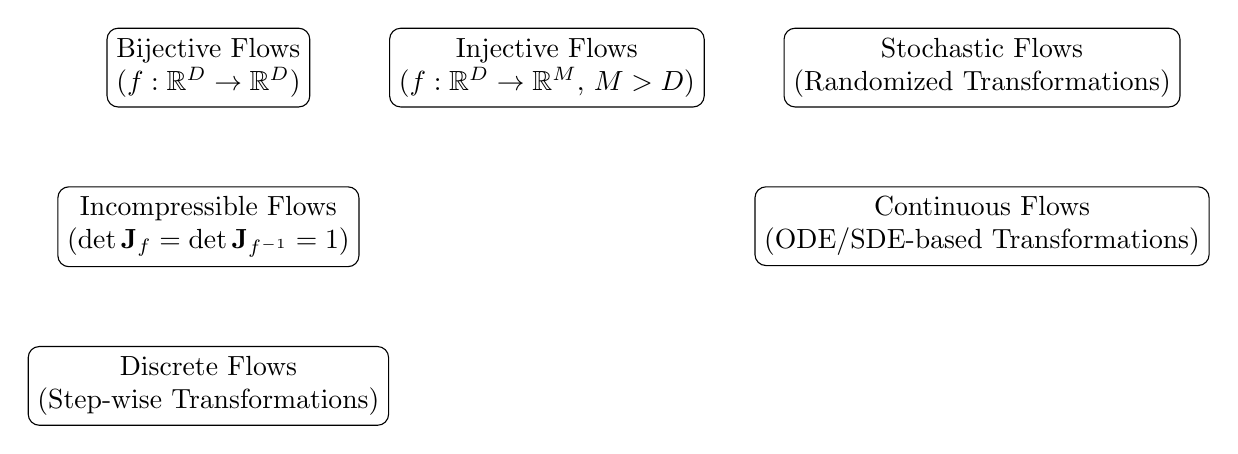
\begin{tikzpicture}[
        every node/.style={draw, align=center, rounded corners, minimum width=2.5cm, minimum height=1cm},
        arrow/.style={->, thick}
    ]
    
    % Nodes
    \node (bijective) {Bijective Flows\\($f: \mathbb{R}^D \to \mathbb{R}^D$)};
    \node [below=of bijective]  (incomp) {Incompressible Flows\\($\det \vJ_f = \det \vJ_{f^{-1}} = 1$)};

    \node[right=of bijective] (injective) {Injective Flows\\($f: \mathbb{R}^D \to \mathbb{R}^M$, $M > D$)};
    \node[right=of injective] (stochastic) {Stochastic Flows\\(Randomized Transformations)};
    \node[below=of incomp] (discrete) {Discrete Flows\\(Step-wise Transformations)};
    \node[below=of stochastic] (continuous) {Continuous Flows\\(ODE/SDE-based Transformations)};
    
    % Arrows
    % \draw[arrow] (bijective) -- (injective);
    % \draw[arrow] (bijective) -- (stochastic);
    % \draw[arrow] (stochastic) -- (discrete);
    % \draw[arrow] (stochastic) -- (continuous);
    % \draw[arrow] (bijective) -- (incomp);

    
    \end{tikzpicture}
\end{center} 


The tipping point for the the Diffusion revolution is to observe that $p(\vx)$ can be a well-defined, easy to sample, easy to model, distribution, while $p(\vz)$ can be an arbitrarily complex distribution, as long as we have a sophisticated transformation $f$ that is smooth and invertible.


Dalton Board as Incompressible flow.


\subsection{Composing Flows into Discrete Flows}
Prior to diffusion, generative models were trying to learn the mapping function from the complex data distribution to some distribution like $\fN(0, I_d)$ that is easy to sample from. VAEs, GANs, etc all mapped the data distribution back to Gaussian noise distribution and tried to lean the inverse mapping. 

The standard way of getting around this problem is to compose different transformations to get a more sophisticated transformation. In other words, we make use of the property that a composition of injective functions is another injective function. 

\begin{align}
    h = f_1 \circ f_2 \circ  \cdots \circ f_K
\end{align}
Where, across $K$ time steps, transformation functions $f_k$ are composed together to construct the final transformation $h$. The corresponding CoV formula would be
\begin{align}
\log p(\vz) = \log p(h^{-1}(\vz)) + \sum_{k=1}^K \log \det \vJ_{f_k} \eqcomment{CoV for Composed Flows} \label{eq:cov-loglik}
\end{align}
Note that we have simply written the CoV formula in terms of log of the probability density so as to make it evident that Normalizing flows can be trained by simply maximizing the above log likelihood.

The DDPM forward process is defined as follows. At $t=0$, $\vx_0 \sim p_{\text{data}}$ and across $T$ time steps, Gaussian noise is added as shown below.

\begin{align}
    \vx_t &= \sqrt{1-\beta_t} \vx_{t-1} + \sqrt{\beta_t}\epsilon; \quad \epsilon \sim \fN(0, I_D) \\
    &= \sqrt{1-\beta_t} \vx_{t-1} + \fN(0, \beta_t I_D) \\
    &\sim \fN(\sqrt{1-\beta_t} \vx_{t-1}, \beta_t I_D) = q(\vx_t | \vx_{t-1})
\end{align}
Where $q(\vx_t | \vx_{t-1})$ is the transition probability density from $\vx_{t-1} \to \vx_t$. We can aggregate the $t$ time steps and write the state $\vx_t$ at time $t$ in terms of the initial data samples $\vx_0$ as
\begin{align}
    \vx_t = \sqrt{\bar{\alpha}_t} \vx_0 + \sqrt{1 - \bar{\alpha}_t} \epsilon
\end{align}
Where $\bar{\alpha}_t = \prod_{i=1}^T (1 -\beta_i)$ and $\epsilon \sim \fN(0, I_D)$. Consequently, the joint distribution of the noisy data $\vx_t$ across $t = 1, \ldots T$ conditioned on the initial data sample $\vx_0$ can be written as

\begin{align}
    q(\vx_1, \ldots, \vx_T | \vx_0) = \prod_{t=1}^T q(\vx_t | \vx_{t-1})
\end{align}
Thus, every transition distribution is Markovian, depending only on its previous state $\vx_{t-1}$.


\subsubsection{Training Discrete Flows}
The discrete flows have sometimes been called \textbf{Variational Diffusion Models} (VDM) \citep{kingma2021variational} for the reason that they were initially trained using the Evidence Blower Bound (ELBO), similar to VAEs.



\begin{align}
    \text{ELBO}(\vx) = \E[\log p(\vx_0 | \vx_1)] - \D_{KL}(q(\vx_T | \vx_0) \| p(\vx_T)) - \sum_{t=2}^T \E[\D_{KL}(q(\vx_{t-1} | \vx_t, \vx_0) \| p(\vx_{t-1}|\vx_t))]
\end{align}


\subsubsection{Issues with Discrete Flows}
So far, the probabilistic flows have been discrete in time.

The difficulty in training such models is that there is no closed-form loss function. The loss function needs to be approximated via an \emph{evidence lower bound} (ELBO).

During training, it is necessary to choose a time-discretization.

Futhermore, the discrete flows require closed-form marginal distributions that are gaussian. As such their forward processes are a special case of probability paths.


In case of continuous time, CFM is not a lower bound to FM but equivalent.


\subsection{Moving from Discrete to Continuous Flows}


\subsubsection{Issues with Continuous Normalizing Flows}

\subsection{Rectified Flows}

\section{Flow Matching Framework}

\subsection{Conditional Flow Matching}

\subsection{Optimal-Transport CFM}

\section{Score Matching Framework}

\subsubsection{Benefit of adding Noise}



\bibliographystyle{unsrtnat} 
\bibliography{references}

\end{document} 